\chapter{Name of chapter}

\lipsum[1] % sample text

Morlet wavelet's are a fascinating subject and quite important for the study of computational neuroscience \cite{COHEN2019}.

% write chapter here

%%%% FIGURES %%%

\begin{figure}[h]
    \centering
    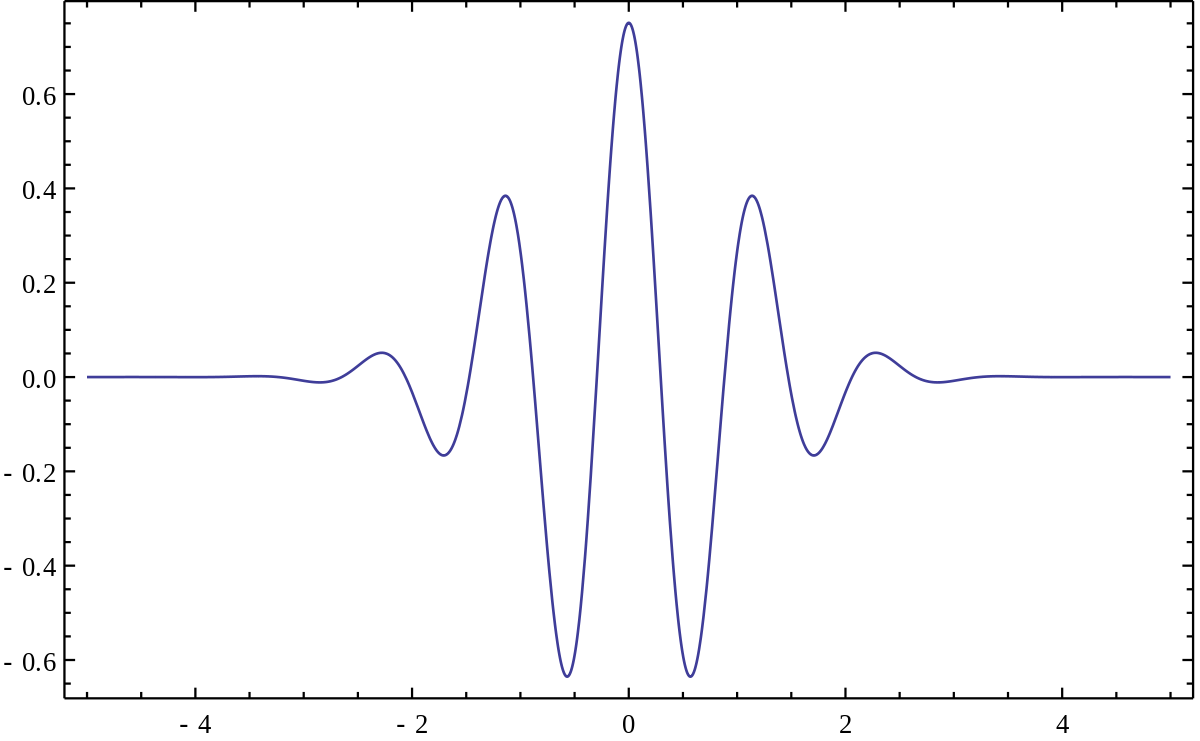
\includegraphics[scale=0.2]{figures/morlet_wavelet.png}
    \caption{Morlet Wavelets}
    \label{fig:morlet}
\end{figure}

A complex morlet wavelet can be derived from the following equation.

%%%% Equation %%%%
\begin{equation}
\label{gausswindow}
    w=e^{2i \pi ft}e^\frac{-t^2}{2\sigma^2}
\end{equation}

Equation \ref{gausswindow} is the product of a sine wave and gaussian window.


